One of the defining properties of topological insulators is the presence of conducting edge states with an insulating bulk. The example considered here in sec. \ref{sec:ti_exemples} is a two dimensionnal material and its edge is therefore one-dimensionnal. The QH and QSH effects both involve one-dimensionnal conduction. In one dimension, electrons can only either move forward of backward on the edge of the sample and this restriction is central for Hall effects. \cite{qi_quantum_2010}. 
\subsection{QH}
The QH effet occurs in two dimensionnal semiconductor electron gas with a strong applied magnetic field \cite{qi_quantum_2010}.

\begin{figure}[h]
    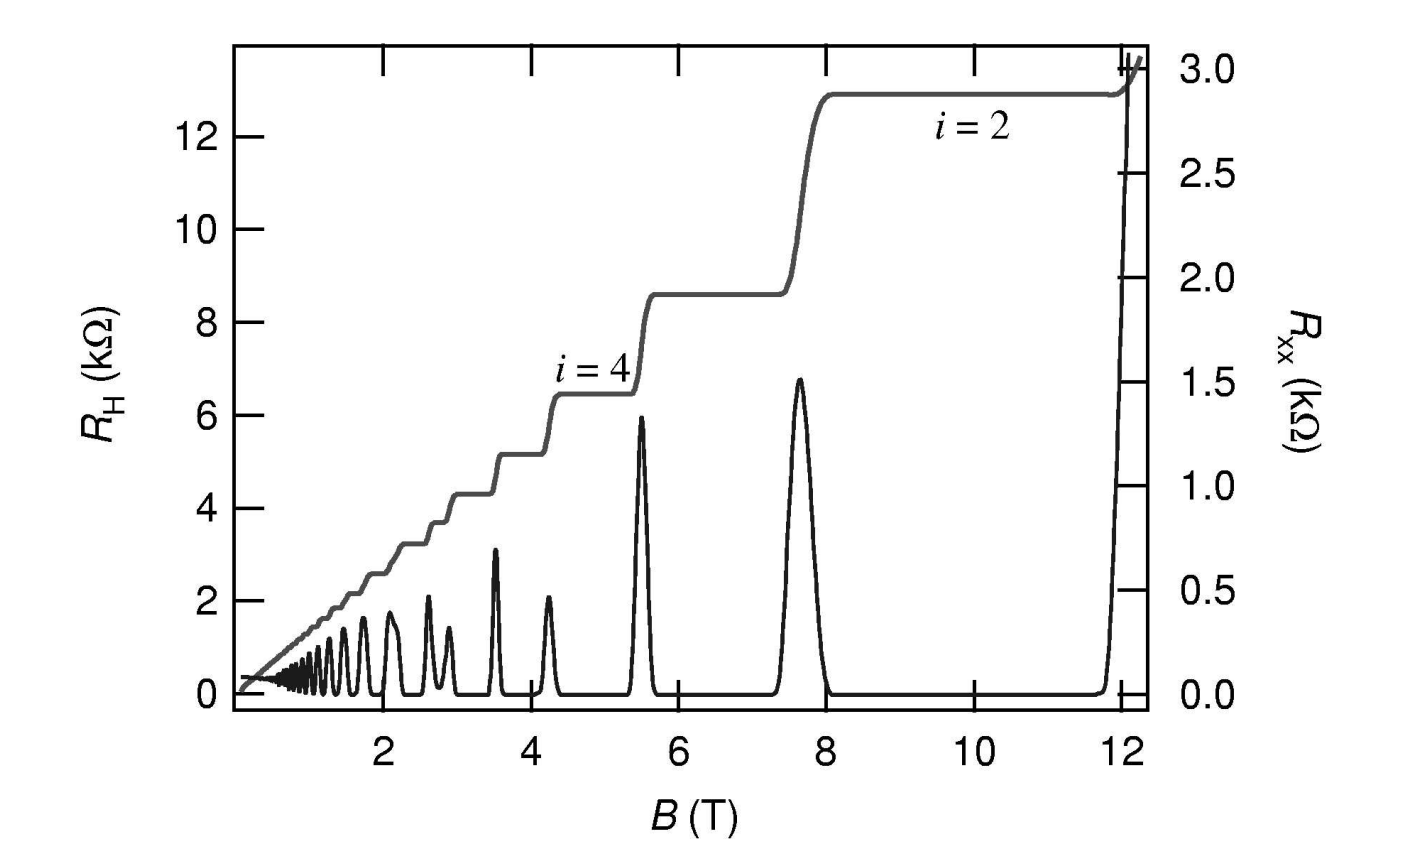
\includegraphics[width=\columnwidth]{sections/visuel/Hall_effect.png}
    \caption{Hall Effect mersurments. The upper curve represent the Hall resistance ($R_h \propto \frac{1}{\sigma_{xy}}$) and shows its plateaus while the lower one represent $R_{xx} \propto \rho_{xx}$ and shows its vanishing. Both curve are a function of the magnetic feild. \cite{jeckelmann_quantum_nodate}}
    \label{fig:Hall_effet}
\end{figure}

It consists of a two simultanious and related phenomena. The quantized \textit{Hall conductivity} $\sigma_{xy}(=\frac{I_x}{V_y})$ and the vanishing of the $\rho_{xx}$ resistivity in a 2D electron gas. The vanishing of $\rho_{xx}$ is due to the existance of edges states.%because the conducting edge states only carry current in one direction on a given side of the sample.
In the case of the Hall effet, such edge state exist beaucse of the discontinuity between the Chern number of the material and the Chern number of empty space. This symetry breaking region implies an unsual asymetric dispersion relation which has forward moving states then backward moving state, imposing conduction along the edges.\cite{kane_topological_2013} These state are resilient since adding an impurity can't lead to backscattering of the electrons because there are simply no backward moving states they can scatter into \cite{qi_quantum_2010}.  The link with topology is fairly direct since the Hall Conductivity is directly proportional to the Chern number! In fact we have.
\begin{equation}
\sigma_{xy} = \mathcal{C}\frac{e^2}{\hbar}
\end{equation}

where $\mathcal{C} \in \mathbb{N}$ is the Chern number.

\begin{figure}[h!]
    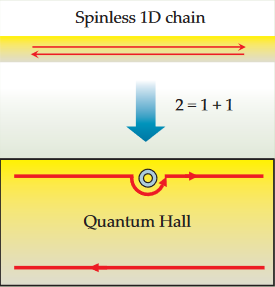
\includegraphics[scale = 0.7]{sections/visuel/spinless.png}
    \caption{Schematic representation of the conduction chanels in a spinless quantum Hall system.\cite{qi_quantum_2010}}
    \label{spinless}
\end{figure}



\subsubsection{Chern number}

% The Chern number is a topological invariant closely related to the Euler characteristic. In fact you can write the \textit{topological solid} equivalent of the \textit{Gauss-bonnet} theorem 



\subsubsection{Impossiblity of backscattering}

\subsubsection{In which material does it happen}


\subsection{QSH}

The QSH state can be obtained from the combination of two copies of the QH state \cite{buhmann_quantum_2011}. In this new state, two counter propagating channels of edge states exist on each side of the sample. Kramer's theorem (see sec. \ref{TRS}) relates these pairs of edge states with TRS \cite{buhmann_quantum_2011}. Since these states are related by TRS, they have oposite crystal momentum $\mathbf{k}$ and spin: they are \textit{helical} edge states \cite{bernevig_topological_2013}. Since helical states couple $\mathbf{k}$ with spin, QSH states can only be realised in systems with strong spi-orbit coupling \cite{qi_quantum_2010}. The number of Kramer pairs of edge states is an exemple of a $\mathbb{Z}_2$ invariant which tells if the state is topological or not \cite{koenig_quantum_2008}. Here, the helical states come in one Kramer pair (taking effect on both sides of the sample), so there is an odd number of Kramer pairs and the $\mathbb{Z}_2$ invariant allows to call the QSH state a topological state of matter.\\

The impossiblity of backscattering on impurities in the QSH state can be directly related to the effect of an antireflection lens \cite{qi_quantum_2010}. The effect of scattering on an impurity is represented in fig. \ref{lens} (B). Two quantum paths can be taken by the electron encountering the impurity. In both cases an helical state must be converted into its Kramer partner by the scattering in order to reverse the direction of motion. When the electron goes around the impurity, its spin turns by an angle of $\pm \pi$ depending on the sens of rotation around the impurity (fig. \ref{lens} (B) up and down show the two possible paths sawpping momentum direction). The global angle difference between the two spin rotations is $2\pi$. Because the phase of half integer particles rotates with half the speed of the actual rotation whitnessed by the electron, the $2\pi$ angle difference becomes a $\pi$ phase shift. A completely destructive interference between the two quantum paths emerges and the backscattering is forbidden. This is just like perfect transmission of an antireflection lens generated by the destructive interference of the red and blue paths of fig. \ref{lens} (A). 

\begin{figure*}
    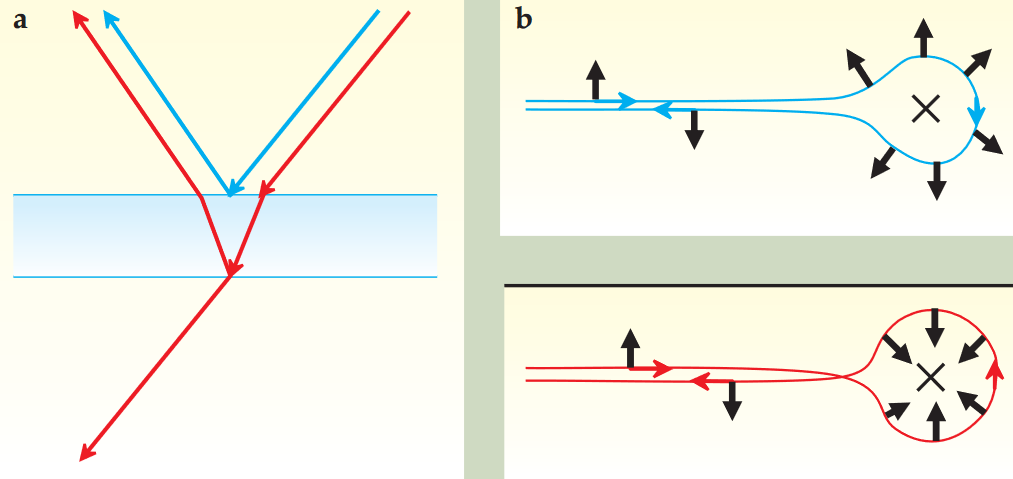
\includegraphics[scale = 0.7]{sections/visuel/lens.png}
    \caption{Analogy between an antireflection lens (A) and the interference phenomena (B) occuring in the QSH state to prevent backscattering on impurities represented by $X$ \cite{qi_quantum_2010}}
    \label{lens}
\end{figure*}



\begin{figure}[h!]
    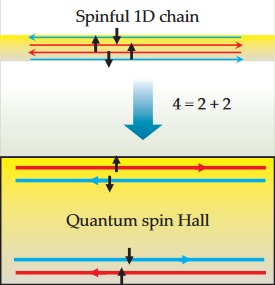
\includegraphics[scale = 0.7]{sections/visuel/spinful.png}
    \caption{Schematic representation of the conduction chanels in a spinlful quantum Hall system.}
    \label{spinful}
\end{figure}

% Talk about the fact that the states are topologicaly protected since their edge states survive the addition of impurities \cite{kane_this_2011}